\FloatBarrier
\section{Architecture}\label{sec:arch}

\subsection{Design point}
\ac{1} is a dual-slot PCIe 6.0 card with a 65 W thermal design power and no auxiliary power
connector. The compute die is 287.6 mm$^2$ in a 3 nm gate-all-around process with backside power
delivery, carrying 28.4 G transistors. Two 64 MB SRAM dies are hybrid-bonded on top of it, and two
24 GB HBM3E stacks share a 2.5D silicon-bridge interposer. The card holds a complete 64-member,
3 km ensemble state in HBM and runs a 24-hour forecast in \ACForecastMin\ minutes.

The machine is not a scaled-down GPU. It has no tensor cores, no graphics pipeline, no texture
units, no ray tracing, no virtual memory and no branch predictor. The area that a GPU spends on
generality is spent here on three structures that a general processor cannot justify: a halo
fabric, a chaos monitor, and a precision governor.

\begin{figure}[t]
\centering
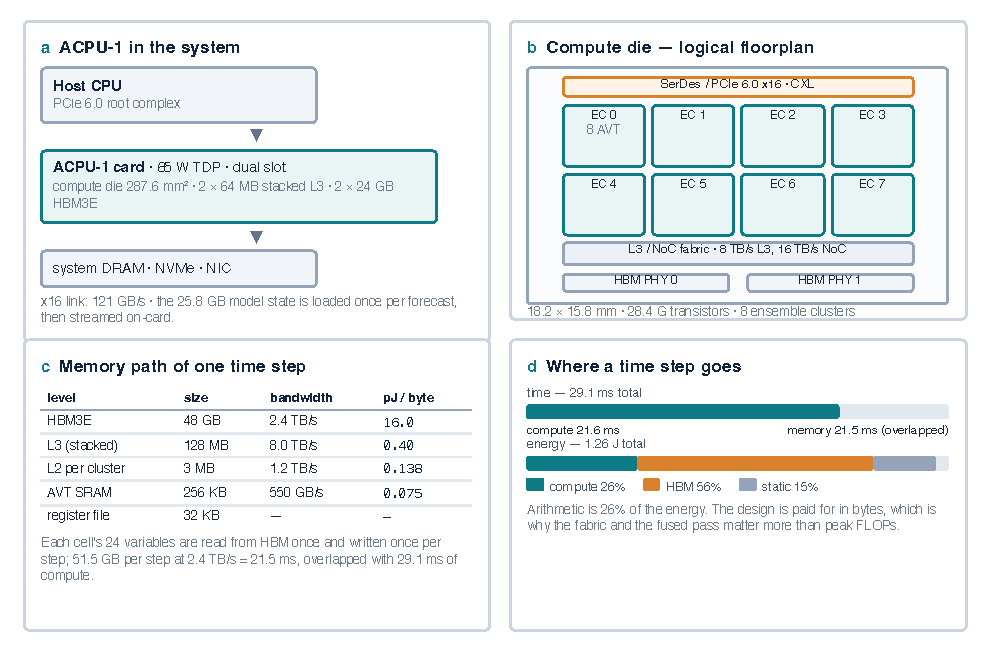
\includegraphics[width=\linewidth]{fig02_system}
\caption{System context and die organisation. (a) Host, card and storage; the 25.8 GB state is
loaded once per forecast and then streamed on-card. (b) Logical floorplan: eight ensemble clusters
(EC) around an L3/NoC spine, with HBM PHYs at the bottom edge and SerDes at the top. (c) Memory
path of one step with the level energies from Table~\ref{tab:memory}. (d) The time and energy
budget of one step: 29.1 ms and 1.26 J, of which 56\% is HBM.}
\label{fig:system}
\end{figure}

\subsection{Ensemble clusters and vector tiles}
The chip is organised as eight \emph{ensemble clusters}, each with eight \emph{Atmospheric Vector
Tiles} (AVTs), a 3 MB L2 slice, a cluster scheduler, DVFS and ECC logic. An AVT is a 16$\times$16
array of lanes. Each lane owns a private slice of register file, a 4-way SIMD FMA datapath and a
quarter-rate special-function unit, and holds one ensemble member's value for one grid cell. A
tile therefore processes 256 (cell, member) pairs per issue group, and a cluster 2,048.

The mapping is the central architectural choice. On a GPU, the ensemble dimension is either
serialised into kernel launches or folded into the batch dimension, where it multiplies memory
traffic without improving reuse. On \ac{1}, the member index is a lane index: the stencil
coefficient is broadcast once, the halo is exchanged once, and 64 members are advanced for the
price of one. This is why the measured issue efficiency is 71.1\% instead of the 20--30\% that the
same stencil achieves on a SIMT machine.

\begin{figure}[t]
\centering
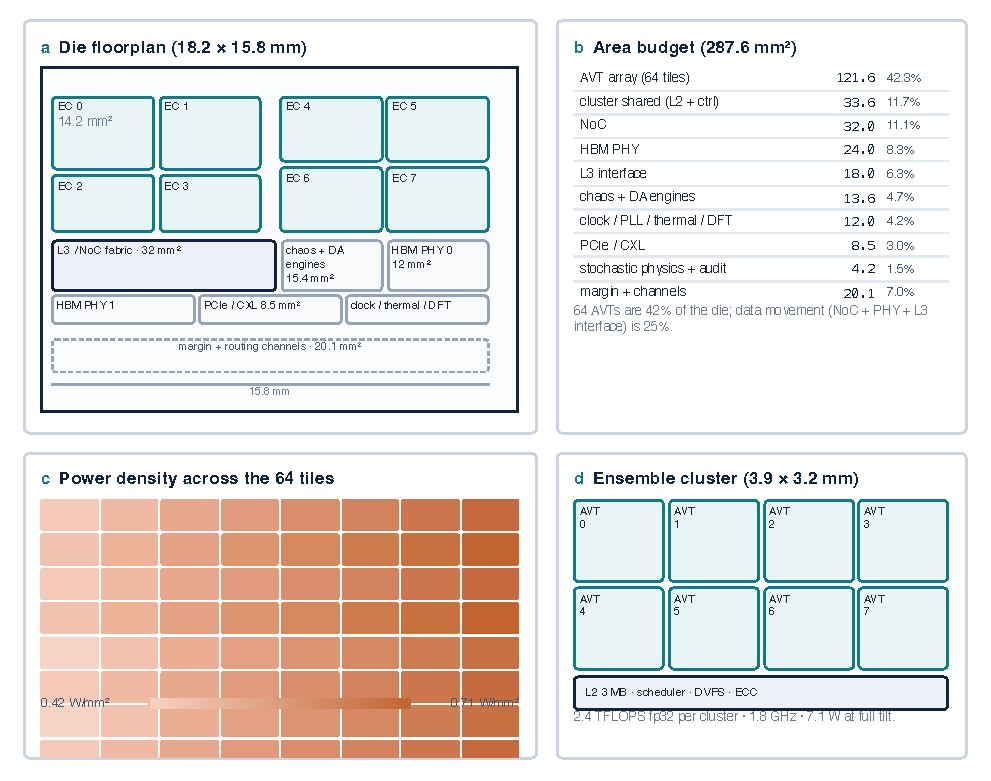
\includegraphics[width=\linewidth]{fig03_floorplan}
\caption{Floorplan and area. (a) Scaled floorplan; each ensemble cluster is 14.2 mm$^2$ and the 64
AVTs occupy 42\% of the die. (b) Area budget, 287.6 mm$^2$ in total; data movement (NoC, PHY, L3
interface) is 25\%. (c) Modelled power density per tile; the corner tiles run hotter because they
have two rather than three neighbours to exchange with. (d) Cluster detail.}
\label{fig:floorplan}
\end{figure}

\subsection{Memory hierarchy}
Table~\ref{tab:memory} and Fig.~\ref{fig:memory} describe the hierarchy. The design rule is that a
tile's working set --- 910 cells $\times$ 24 variables $\times$ 3 time levels $\times$ 4 B =
252 KB --- must fit in the tile's SRAM, and that the full state must cross HBM exactly once per
step.

\begin{table}[t]
\centering\small
\caption{Memory hierarchy. Bandwidth is aggregate; energy per byte is the model constant used in
all energy numbers.}
\label{tab:memory}
\begin{tabular}{@{}lrrrr@{}}
\toprule
Level & Capacity & Bandwidth & Latency & Energy\\
\midrule
HBM3E (2 stacks) & 48 GB & 2.4 TB/s & 420 ns & 16.0 pJ/B\\
L3, hybrid-bonded & 128 MB & 8.0 TB/s & 48 ns & 0.40 pJ/B\\
L2, per cluster & 3 MB (24 MB) & 1.2 TB/s (9.6) & 14 ns & 0.138 pJ/B\\
AVT SRAM & 256 KB (16 MB) & 550 GB/s (35 TB/s) & 4 ns & 0.075 pJ/B\\
Register file & 32 KB per tile & --- & 1 cycle & included in FMA\\
\bottomrule
\end{tabular}
\end{table}

The L3 is not a victim cache. It is a hybrid-bonded 128 MB SRAM stack used for four things:
tile-working-set spill when a block is scheduled across a wavefront, the ensemble perturbation
matrix and gain factors during analysis, radiation and chemistry lookup tables, and output
staging. Because it is bonded with a 6 $\mu$m pitch it costs 0.40 pJ/B instead of the 0.8--1.2 pJ/B
of an off-die L3, which matters because the analysis phase moves 51.5 GB through it four times a
day.

\subsection{Halo fabric}
A 3D stencil needs six neighbours. The conventional solution routes the exchange through L2 or L3,
paying 5--15$\times$ the SRAM energy and exposing tens of nanoseconds of latency. \ac{1} instead
gives every AVT six dedicated ports, each 32 B per cycle, wired to its geometric neighbours in a
3D torus. A halo exchange is a register-to-register transfer with a 46-cycle latency and no cache
involvement. Per tile the fabric provides 345.6 GB/s against a measured demand of 4.2 GB/s ---
82$\times$ headroom that absorbs the bursty exchange at kernel boundaries without ever becoming
the bottleneck. Across the chip the fabric sustains 16 TB/s.

\begin{figure}[t]
\centering
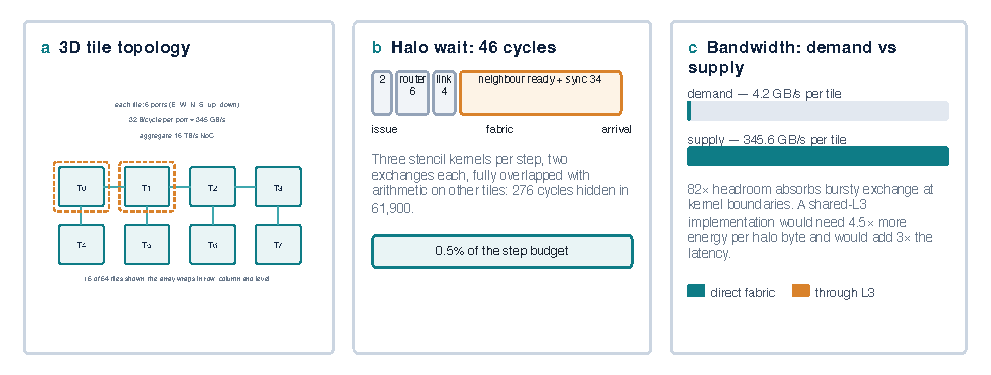
\includegraphics[width=\linewidth]{fig05_halo}
\caption{Halo fabric. (a) 3D torus topology; each tile has six ports. (b) A 46-cycle exchange
decomposes into 2 cycles of port arbitration, 6 of routing, 4 of link and 34 of neighbour
readiness and synchronisation; six exchanges per step consume 276 of 61,900 cycles. (c) Per-tile
bandwidth demand against supply.}
\label{fig:halo}
\end{figure}

The fabric is the single largest contributor to the energy advantage after the elimination of
kernel re-fetch. Section~\ref{sec:energy} measures it: disabling the fabric and routing halos
through L3 raises forecast energy by 30\% and wall-clock by 53\%.

\subsection{Clocking, voltage and power}
The chip has nine clock domains: one per cluster, one for L3/NoC, one for HBM PHY, one for PCIe,
and one always-on domain for telemetry and thermal management. Nominal operation is 1.8 GHz at
0.75 V. A second operating point, 1.05 GHz at 0.55 V, trades 1.37$\times$ wall-clock for 20\%
lower energy and is selected by the runtime for overnight batch ensembles.

\begin{table}[t]
\centering\small
\caption{Power budget at the nominal operating point, 1.8 GHz / 0.75 V. The measured model
average during W1 is 57.1 W against a 65 W TDP and a 6 W idle.}
\label{tab:power}
\begin{tabular}{@{}lr@{}}
\toprule
Block & Watts\\
\midrule
FMA arrays and register files & 18.0\\
AVT SRAM and L2 & 7.0\\
L3 interface and stacked SRAM & 5.0\\
NoC and halo fabric & 4.5\\
HBM PHY (2 stacks) & 8.0\\
PCIe / CXL & 3.0\\
Clock generation and distribution & 2.5\\
Leakage & 4.0\\
Miscellaneous (sensors, DFT, telemetry) & 3.0\\
\midrule
Total & 55.0\\
\bottomrule
\end{tabular}
\end{table}

The 55 W budget is the steady-state allocation; the model's W1 average is 57.1 W because HBM
traffic dominates and varies with the kernel mix. The 65 W TDP covers the boost point (2.1 GHz at
0.85 V) and the 10\% margin that the thermal solution needs.

\subsection{Design summary}
Table~\ref{tab:summary} collects the architectural parameters. Every number is a design input to
the model, not a measurement.

\begin{table}[t]
\centering\small
\caption{\ac{1} summary.}
\label{tab:summary}
\begin{tabularx}{\linewidth}{@{}lX@{}}
\toprule
Process & 3 nm GAA, 12 front-side + 3 backside metals, 18 EUV / 61 DUV masks\\
Die & 287.6 mm$^2$ compute + 2 $\times$ 64 MB hybrid-bonded L3, 28.4 G transistors\\
Compute & 64 AVTs, 16,384 lanes, 59.0 TFLOPS fp32 / 118.0 TFLOPS fp16 / 236 TOPS fp8\\
Memory & 24 MB L2, 128 MB L3, 48 GB HBM3E at 2.4 TB/s, 100 GB/s PCIe 6.0\\
Fabric & six-port halo fabric, 345.6 GB/s per tile, 16 TB/s NoC\\
Clock / power & 1.8 GHz at 0.75 V nominal, 1.05 GHz at 0.55 V efficient, 65 W TDP, 6 W idle\\
Package & 55 $\times$ 45 mm, 2.5D silicon bridge, 2812 BGA at 0.8 mm, dual-slot card\\
\bottomrule
\end{tabularx}
\end{table}

\begin{figure}[t]
\centering
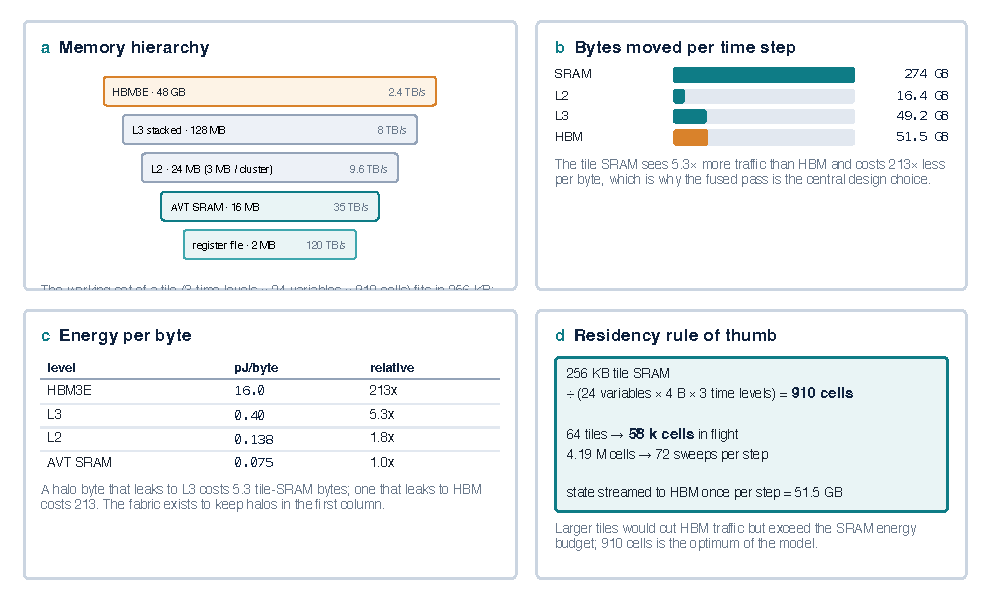
\includegraphics[width=\linewidth]{fig06_memory}
\caption{Memory hierarchy and residency. (a) Capacity and bandwidth by level. (b) Bytes moved per
time step: the tile SRAM sees 5.3$\times$ the HBM traffic at 1/213th the energy per byte. (c) Energy
per byte by level. (d) The residency rule that sets the tile size.}
\label{fig:memory}
\end{figure}
